In this section, we analyze region-wide trends in accessibility losses for the case study area. As mentioned in Section~\ref{sec:accIntro}, we first analyze each of the 12 socio-economic groups used in practice for the case study region~\cite{ory_personal_2013}, which are characterized based on households. The socio-economic groups correspond to all combinations of four different income classes (Table~\ref{tab:incomes}),
%(low (0 - \$25,000 in 1989 USD, 0 - \$47,334 in 2014 USD), medium (\$25,000 - \$45,000 in 1989 USD, \$47,334 - \$85,202 in 2014 USD), high (\$45,000 - \$75,000 in 1989 USD, \$85,202 - \$142,004 in 2014 USD), very high (more than \$75,000 in 1989 USD, \$142,004 in 2014 USD)), 
and three different classes of automobile availability in the household (zero automobiles, fewer automobiles than household members that work, a greater or equal number of automobiles as compared to the number of household members that work).


%These are classified by the income class and the relative number of vehicles (``cars'') to the number of household members that work as follows: a) low income, no cars, b) low income, workers $<$ cars, c) low income, workers $\geq$ cars, d) medium income, no cars, e) medium income, workers $<$ cars, cf) medium income, workers $\geq$ cars, g) high income, no cars, h) high income, workers $<$ cars, i) high income, workers $\geq$ cars, j) very high income, no cars, k) very high income, workers $<$ cars, and l) very high income, workers $\geq$ cars. Note, that very high income corresponds to households with a combined income of greater than \$142,004 USD (2014). Thus, for a given household, we can classify it into a socio-economic group by knowing the income class and the ratio of number of people working to the number of vehicles.

We first assess the data availability for each of the segments. Each data point represents a trip by a person of a household, who is  modeled as an agent in the high-fidelity transportation model. The results suggest comparing households with at least one car, because for households without cars (no cars), only the low income class has reasonably many trips (Figure~\ref{fig:car}). 

%For the other income classes, the corresponding socio-economic groups of no car households is very small. 

%Thus, by themselves, the results from the other three socio-economic groups may not be fully representative of the true dynamics. However, the other nine socio-economic groups have a more reasonable representation. 


\begin{figure}[h]
\centering
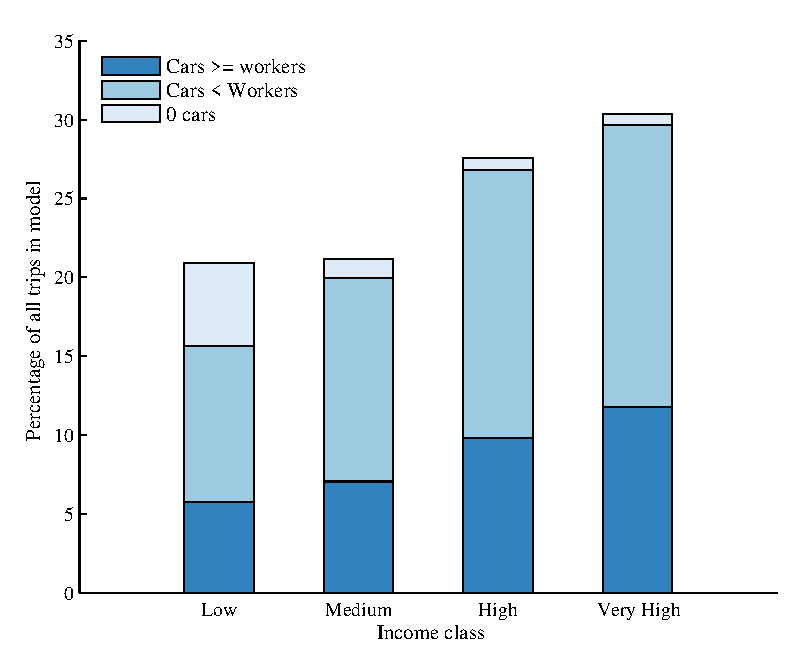
\includegraphics[width=6in]{FIGS/equity_dataset_count_bars.eps} 
\caption{Percentage of total number of trips considered in the high-fidelity model by socio-economic group (determined by income class and household car ownership category) for the baseline (pre-earthquake) case.}
\label{fig:car}
\end{figure}


%maps of socio-economic groups
 
\begin{figure*}[h!]
    \centering
%    \begin{tabular}{ccc}
%    \includegraphics[height=0.2\textheight]{../FIGS/Low_Inc_NoCar_Diff.pdf} &
%    \includegraphics[height=0.2\textheight]{../FIGS/Low_Inc_LT_Diff.pdf} &
%    \includegraphics[height=0.2\textheight]{../FIGS/Low_Inc_GE_Diff.pdf} \\
%         (a) low , no cars & (b)  low, workers $<$ cars & (c) low, workers $\geq$ cars \\
%    \includegraphics[height=0.2\textheight]{../FIGS/Med_Inc_NoCar_Diff.pdf} &
%    \includegraphics[height=0.2\textheight]{../FIGS/Med_Inc_LT_Diff.pdf} &
%    \includegraphics[height=0.2\textheight]{../FIGS/Med_Inc_GE_Diff.pdf} \\
%             (d)  medium, no cars & (e) medium, workers $<$ cars  & (f) medium, workers $\geq$ cars \\
%    \includegraphics[height=0.2\textheight]{../FIGS/High_Inc_NoCar_Diff.pdf} &
%    \includegraphics[height=0.2\textheight]{../FIGS/High_Inc_LT_Diff.pdf} &
%    \includegraphics[height=0.2\textheight]{../FIGS/High_Inc_GE_Diff.pdf} \\
%             (g)  high, no cars & (h) high, workers $<$ cars & (i)  high, workers $\geq$ cars\\
%    \includegraphics[height=0.2\textheight]{../FIGS/VHigh_Inc_NoCar_Diff.pdf} &
%    \includegraphics[height=0.2\textheight]{../FIGS/VHigh_Inc_LT_Diff.pdf} &
%    \includegraphics[height=0.2\textheight]{../FIGS/VHigh_Inc_GE_Diff.pdf} \\
%             (j)  very high, no cars & (k)  very high, workers $<$ cars & (l)  very high, workers $\geq$ cars\\
%    \end{tabular}
    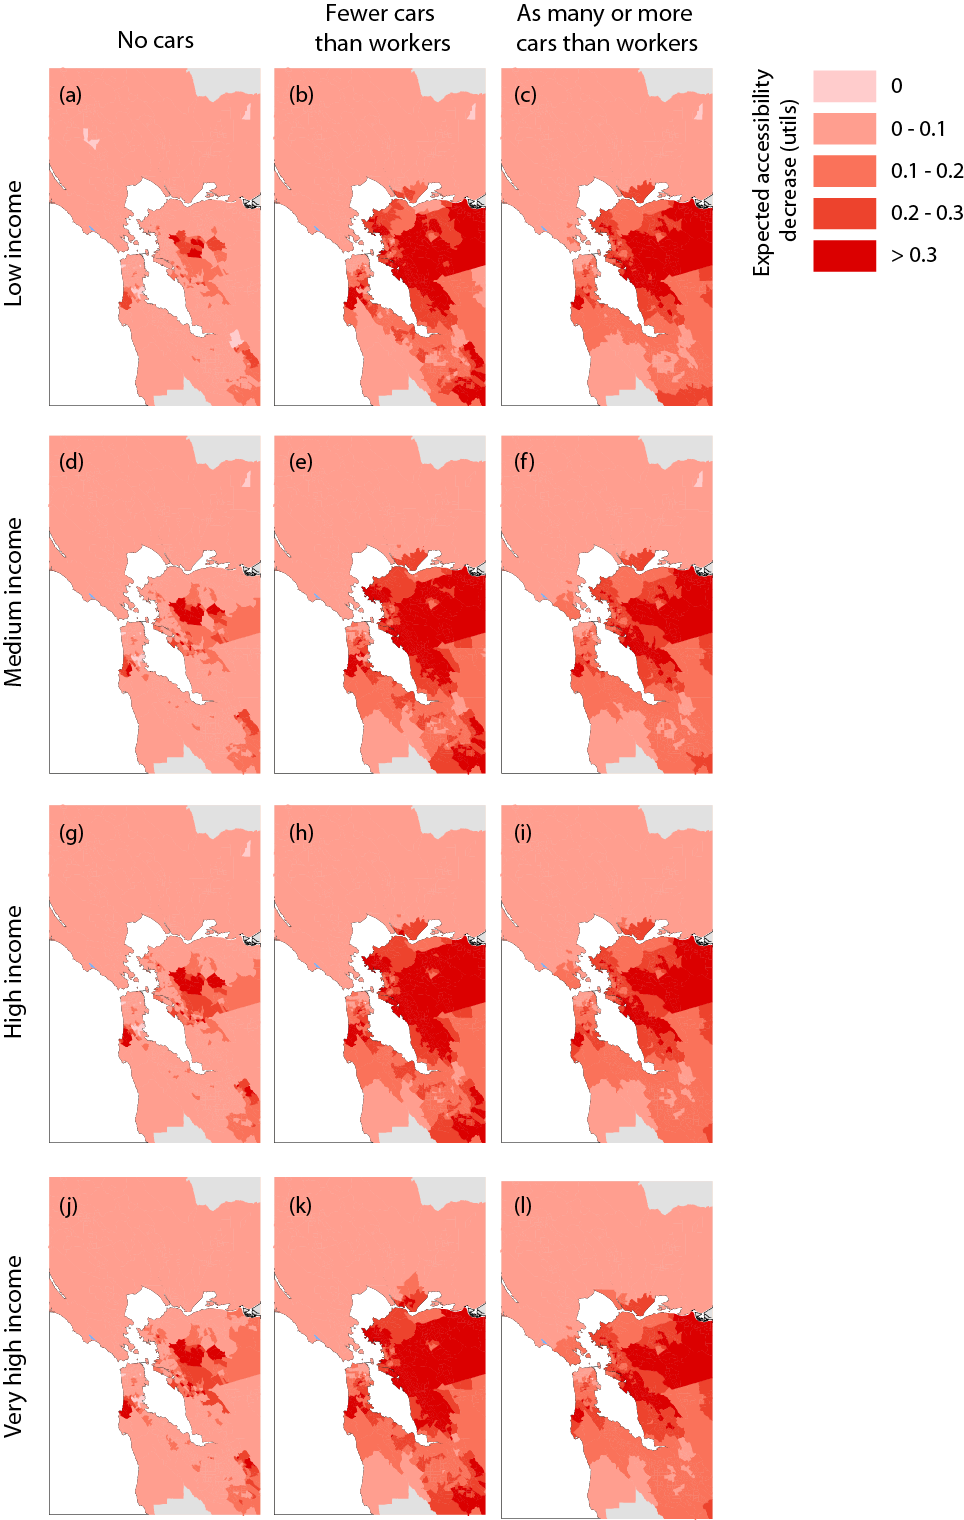
\includegraphics[height=8in]{FIGS/accByGroup.pdf}
\caption{Expected changes in accessibility per person per day for each combination of income class and car ownership group. The darker the color, the greater the losses in accessibility.}% (no cars, workers $<$ cars , workers $\geq$ cars }
%: a) low income, no cars, b) low income, workers $<$ cars, c) low income, workers $\geq$ cars, d) medium income, no cars, e) medium income, workers $<$ cars, cf) medium income, workers $\geq$ cars, g) high income, no cars, h) high income, workers $<$ cars, i) high income, workers $\geq$ cars, j) very high income, no cars, k) very high income, workers $<$ cars, l) very high income, workers $\geq$ cars}
\label{fig:acc_by_segment}
\end{figure*}


General patterns emerge in the expected losses in accessibility.
The expected losses are computed by taking an average of the accessibility results for each of the 1454 travel analysis zones (TAZ) for each earthquake event, weighted by the adjusted annual likelihood of occurrence from the optimization results. 

First, we notice that the ratio of cars to the number of people who work in a household is  correlated with accessibility risk; a higher ratio corresponds to higher expected decreases in accessibility. This corresponds to going across a column in Figure~\ref{fig:acc_by_segment}. For example, for the first row representing low income households, 
 we notice a marked change in accessibility across the columns, as indicated by an expanded area of darkened TAZs from left to right (Figure~\ref{fig:acc_by_segment}{(a-c)}). Note that 1 $util$ corresponds to a consumer value of compensating variation of approximately \$20 per person per day, which assumes low (conservative) estimates of the value of time for travel delays and value of getting to destinations (Section~\ref{sec:accessibility}). 
 
We might expect these households with more cars to take longer trips because there might be a relationship between needing to travel longer distances and needing an extra car or two in a household. This is indeed the case (Figure~\ref{fig:lengthIncomeBars}{(b)}), but it is not fully predictive. In fact, there is only a weak trend between average trip length for a TAZ before any earthquake and the predicted impact on accessibility (Figure~\ref{fig:accLength}). Instead, we hypothesize that there are other latent variables correlated with car ownership. For example, the geographic distribution of people without cars varies. Additionally, in Section~\ref{sec:accDisc}, we will further explore the correlation between the percentage of car-based trips and accessibility risk. We will show that TAZs with fewer car-based trips, tend to have lower risk of accessibility losses.



\begin{figure}[h!]
\centering
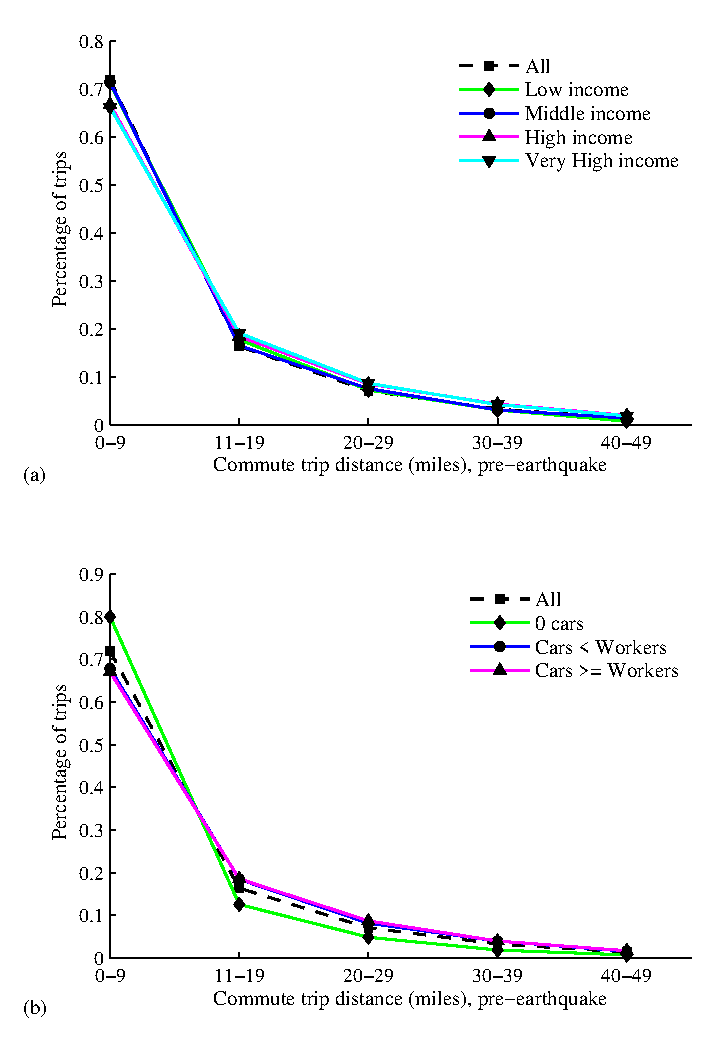
\includegraphics[width=5in]{FIGS/equity_trip_distance_income_cars_to_and_from_work.eps} 
\caption{Distributions of commute trip length in 10-mile intervals  by a) income class segment, and b) car ownership segment,  (pre-earthquake)}
\label{fig:lengthIncomeBars}
\end{figure}

%\subsection{Impact of trip length}
%
\begin{figure}[h!]
\centering
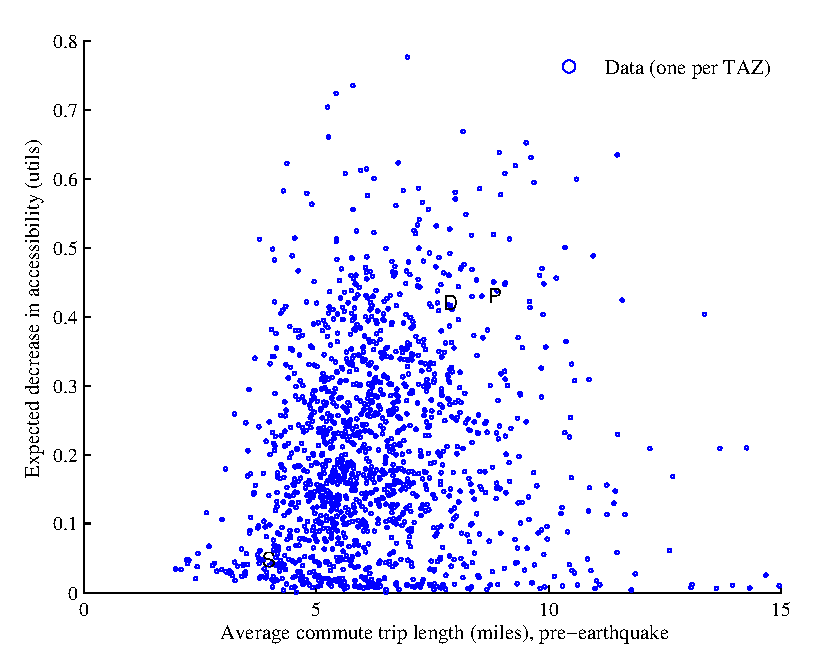
\includegraphics[width=6in]{FIGS/equity_accLength2.eps} 
\caption{Trip length (pre-earthquake) versus change in total accessibility per person per day. Each dot represents one TAZ and the three case study communities, San Francisco financial district, Danville, and Pacifica are marked by \textbf{S}, \textbf{D}, and \textbf{P} respectively.}
\label{fig:accLength}
\end{figure}



Second, controlling for car ownership, we see a fairly equitable distribution of risk across income class segments.  For example, by looking at households with fewer workers than cars (middle column of Figure~\ref{fig:acc_by_segment}), the variation from TAZ to TAZ is significantly more striking than the difference across income segments (Figure~\ref{fig:acc_by_segment}{(b,e,h,k)}). Similarly, while trip lengths are slightly longer for higher income households, the differences are subtle (Figure~\ref{fig:lengthIncomeBars}{(a)}).


Thus, for a given TAZ, the differences across incomes are not that great. At the same time though, there is an unequal geographic distribution of wealth in the San Francisco Bay Area. Because of this, when we aggregate accessibility risk across TAZs, we see that accessibility risk rises with increasing household income  (Figure~\ref{fig:acc_by_TAZ_and_income}{(b)}). Therefore, even though the poor are generally the most vulnerable to climatological and geophysical hazards and disasters including hurricanes, floods and earthquakes~\cite{fothergill_race_1999},  wealthier households in the San Francisco Bay area are more vulnerable than the other income groups to earthquake-related accessibility risk.


%we observe a gradual increase in expected accessibility losses down a column, such as down the right-hand column, representing households where the number of workers is greater than or equal to the number of cars (Figure~\ref{fig:acc_by_segment}{(c,f,i,l)}). However, this trend is more subtle than the trend with car ownership for a fixed income class.





Next, we consider which geographic parts of the San Francisco Bay Area are at an elevated risk. The results show regions of high risk: in the East Bay due East of San Francisco, in the suburbs of San Jose, along the coastal and Bay-side regions South of San Francisco (Millbrae and Pacifica, e.g.), and in parts of San Francisco (South-Central neighborhoods including Westland Highlands and Glen Park neighborhoods) (see labeled map in Figure~\ref{fig:faultsB}). One may have expected more high risk areas on the San Francisco Peninsula, because of the San Andreas fault, which can generate large magnitude events. In contrast, the East Bay has higher shaking levels at more moderate return periods, due to the higher relative annual frequency of events on the Hayward Fault; this is correlated to bridge damage and thus road closures. Furthermore, the data suggests that both the more common moderate-magnitude East Bay events and the rare higher-magnitude San Andreas events can cause accessibility problems for the East Bay. Figure~\ref{fig:scen_acc} shows one sample realization of a M6.85 Hayward event and one sample realization of a M7.45 San Andreas event---both follow the general trend of  high predicted accessibility losses in the East Bay.
%In contrast, the more moderate, more frequent Hayward event caused little impact for San Francisco; the San Andreas events were the chief contributors to the loss of accessibility in San Francisco. 
In contrast, while any events could contribute to the risk in San Francisco, our model results show the main accessibility losses in San Francisco corresponding to the San Andreas events.
Figures~\ref{fig:scen_acc}{(c,d)} provide one such example. Figures~\ref{fig:scen_acc}{(e,f)} show an example of a lower magnitude event farther away from the main population centers, a M6.35 event in the Great Valley Pittsburg-Kirby Hills Fault. This shows how the range of more minor faults in the East Bay can contribute to that area's risk.
%, e.g., Figures~\ref{fig:scen_acc}{(d,f)}. 
%Note that in the three individual earthquake events shown---Hayward, M6.85, b) San Andreas, M7.45, c) San Andreas, M8.25---the accessibility losses are higher than average, since these are major events. 
Also, we have shown the results for one socio-economic group in Figure~\ref{fig:scen_acc}, but the other socio-economic groups follow the same general patterns, albeit with different specific values.


%\begin{figure}
%\centering
%\includegraphics[width=\textwidth]{../FIGS/equity_154_198_196.pdf} 
%\caption{Expected changes in accessibility for individual scenarios: a) Hayward, M7.05 (medium income, workers $<$ cars), b) San Andreas, M7.05 (medium income, workers $<$ cars), c) San Andreas, M8.25 (medium income, workers $<$ cars)}
%\label{fig:scen_acc}
%\end{figure}
\begin{figure*}[t]
    \centering
%    \begin{tabular}{cc}
%        \includegraphics[height=0.2\textheight]{../FIGS/bridge_scen_152.eps} &
%    \includegraphics[height=0.2\textheight]{../FIGS/equity_152.pdf} \\
%    (a) Hayward, M6.85 bridge damage & (b) Hayward, M6.85 accessibility losses \\
%            \includegraphics[height=0.2\textheight]{../FIGS/bridge_scen_204.eps} &
%    \includegraphics[height=0.2\textheight]{../FIGS/equity_204.pdf} \\
%    (c) San Andreas, M7.45 bridge damage & (d) San Andreas, M7.45 accessibility losses \\
%            \includegraphics[height=0.2\textheight]{../FIGS/bridge_scen_1423.eps} &
%    \includegraphics[height=0.2\textheight]{../FIGS/equity_1423.pdf} \\
%    (e) Great Valley, M6.35 bridge damage & (f) Great Valley, M6.35 accessibility losses \\
%        \includegraphics[height=0.2\textheight]{../FIGS/equity_probDamageBig.eps} &
%            \includegraphics[height=0.2\textheight]{../FIGS/Med_Inc_LT_Diff.pdf} \\
%    (g) Expected bridge damage (all events) & (h) Expected accessibility losses (all events)\\
%    \end{tabular}
        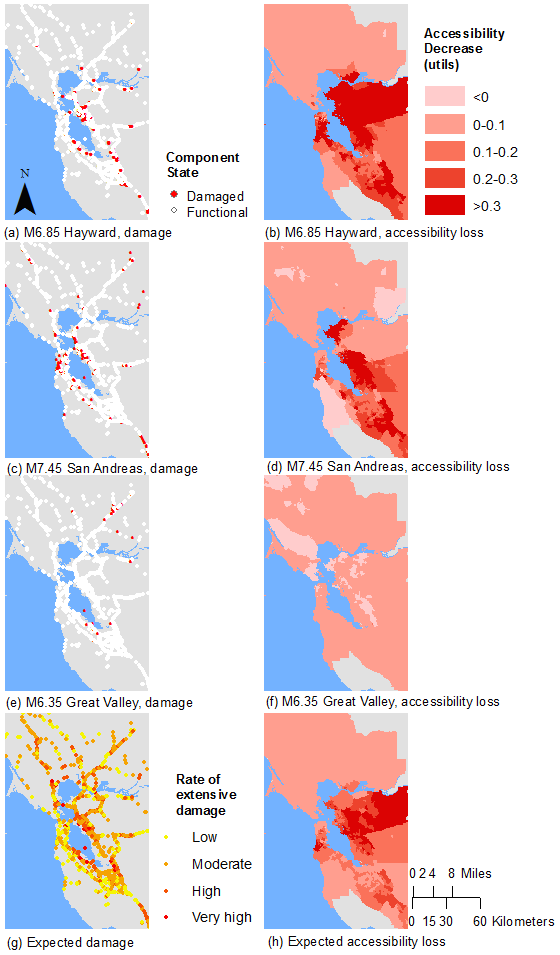
\includegraphics[height=8in]{FIGS/accByEq.png}
    \caption{Bridge damage (red = damaged) and corresponding accessibility losses per person per day by TAZ for medium income households with fewer cars than workers. The bottom row has expected values calculated as a weighted average over all events.}
    % (the darker the color, the greater the losses). For expected bridge damage, the values are on a continuous scale from white to yellow to red in order of increasing annual likelihood of extensive or complete damage.}
\label{fig:scen_acc}
\end{figure*}


% loss exceedance curve
Finally, we can examine the rates of loss exceedance (Section~\ref{sec:theoryMet}). Figure~\ref{fig:acc_by_TAZ_and_income} shows a similar shape to the loss exceedance curves for other performance metrics (Section~\ref{sec:metPM}). Note that the results are primarily valid in the 100 to 2475 year return periods, since this is the range chosen for the map selection optimization problem. As a sense of scale, if we use the average value over all TAZs for this 

Recognizing that the impact varies significantly by TAZ, as indicated by Figure~\ref{fig:acc_by_segment},
%and the general lognormal shape of the accessibility cumulative distribution functions for a given event (Figure~\ref{fig:xxxx})
we also examine the accessibility loss exceedance curve for three communities: part of the San Francisco financial district, Danville, and Pacifica (Figure~\ref{fig:equity_study_area}). These correspond to TAZ IDs 2, 1161, and 224 respectively. This part of the San Francisco financial district  represents an area with relatively low expected changes in accessibility (Figure~\ref{fig:acc_by_segment}), whereas Danville and Pacifica are at an elevated risk in almost all socio-economic groups (Figure~\ref{fig:acc_by_segment}). 
The general trends are corroborated by the loss exceedance curves for these three communities (Figure~\ref{fig:acc_by_TAZ_and_income}{(a)} shows an example for the socio-economic group with medium income households with fewer cars than workers). In other words, the average middle-class person from Danville in a household with fewer cars than people who work is expected to experience travel-related losses up to 1 $utils$ per day after a rare earthquake, which he or she values at approximately \$20 per day considering a conservative estimate of travel time and destination value (Section~\ref{sec:accessibility}). In contrast, his or her fellow Bay Area resident in San Francisco has expected losses of only a tenth as much as experienced by a Danville resident. At return periods greater than 100 years, we notice that Danville and Pacifica follow a similar general pattern, which differs dramatically from that of San Francisco. 

\begin{figure}
\centering
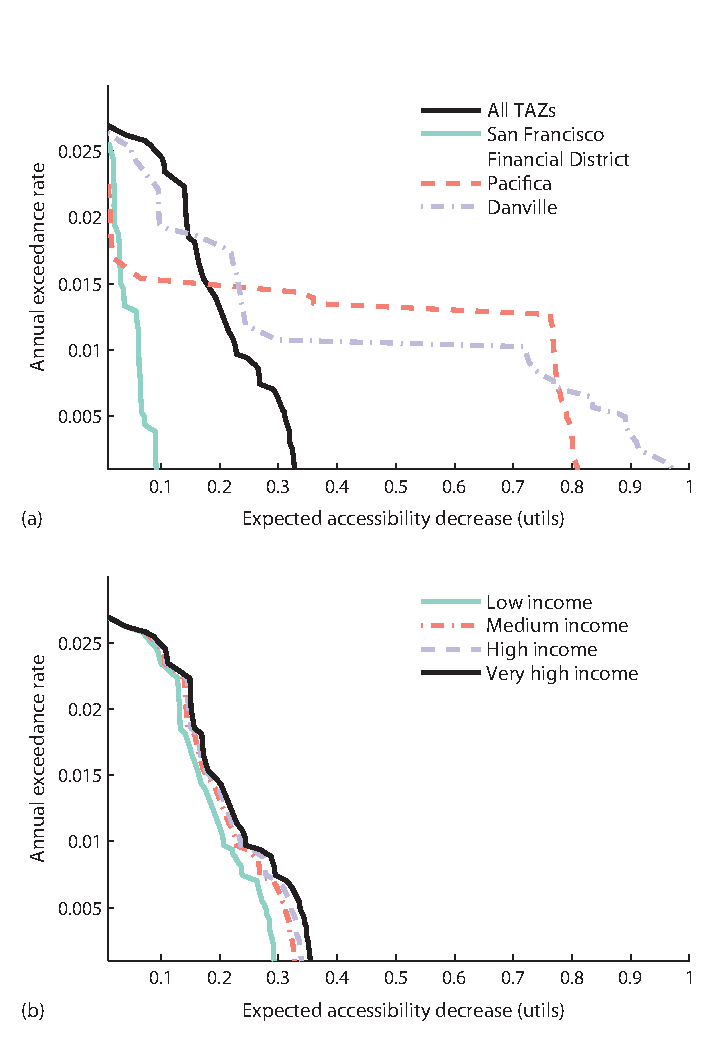
\includegraphics[width=5in]{FIGS/equity_acc_loss_curves.eps} 
\caption{Accessibility annual loss exceedance curve with a comparison by (a) case study TAZs and average over all TAZs and (b) income class; all curves are in $utils$ per person per day for medium income households with fewer cars than workers .}
\label{fig:acc_by_TAZ_and_income}
\end{figure}
